Els plàstics centellejadors són plàstics dopats amb molècules fluorescents, els quals són utilitzats per detectar les partícules d'interés. Aquests es poden mecanitzar de moltes formes diferents, d'entre les quals, l'emprada pel projecte TRITIUM és la fibra ($1~\mm$ o $2~\mm$ de diàmetre i $20~\cm$ de longitud utilitzada en el detector de triti) i el bloc ($17\times 45 \times 1 ~\cm^3$ utilitzada en el vecto actiu). 

En els plàstics centellejadors, les partícules que els travessen depositen part de la seua energia cinètica, la qual excita els electrons de les molécules fluorescents. Finalment aquests electrons es desexciten en nanosegons mitjançant un procés anomenat fluorescència, a través del qual emeten fotons a una longitud d'ona que pertany a l'espectre visible. Aquest espectre d'emissió presenta un pic centrat a una longitud d'ona que depén de la molècula fluorescent. En el cas dels plàstics centellejadors utilitzats en el projecte TRITIUM, la molècula fluorescent conté fluor, el qual presenta un pic d'emissió al voltant de $435~\nano\meter$, com es pot comprovar en la Figura \ref{fig:EspectreEmisioPlasticsTRITIUM}.
\begin{figure}
\centering
    \begin{subfigure}[b]{0.7\textwidth}
    \centering
    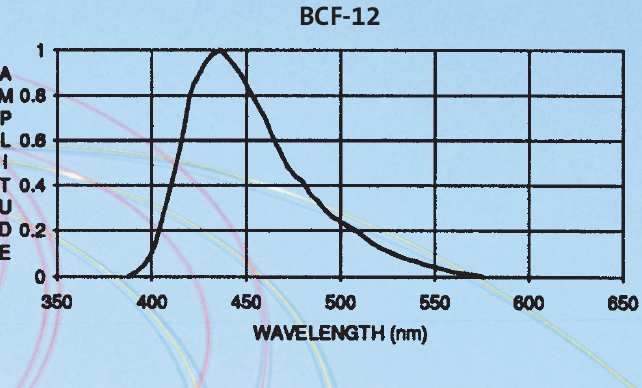
\includegraphics[width=\textwidth]{12Summary/3DesignPrinciples/32Tritium_detector/EmisionBCF12.png}  
        \caption{}\label{subfig:EspectreEmisioFibres}
    \end{subfigure}
    \hfill
    \begin{subfigure}[b]{0.7\textwidth}
    \centering
    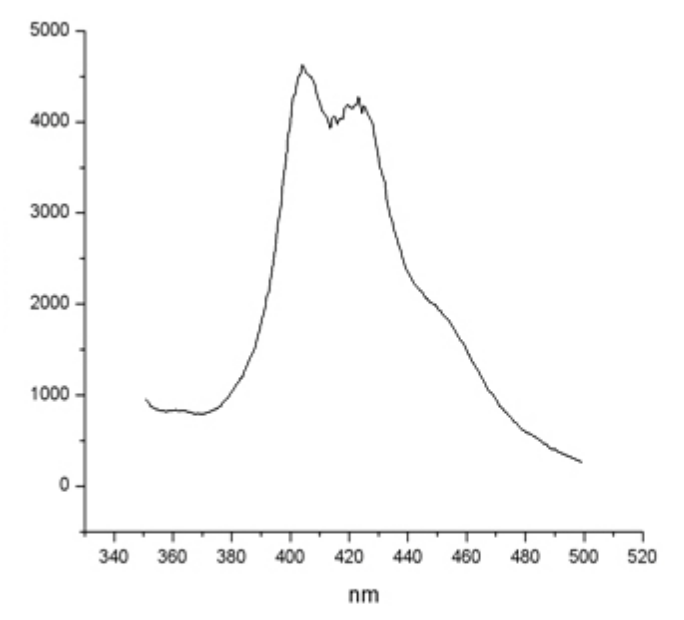
\includegraphics[width=\textwidth]{12Summary/3DesignPrinciples/34BackgroundRejectionSystem/EmissionEnergySpectrumVetos.png}  
    \caption{\label{subfig:EspectreEmisioVeto}}
    \end{subfigure}
\caption{Espectre d'emissió de a) les fibres centellejadores de Saint Gobain, model BCF-12, utilitzades en el detector de triti \cite{DataSheetBCF12Fiber} b) bloc de plàstic centellejador d'Epic Crystals utilitzat en el sistema de rebuig del fons radioactiu\cite{ScintillatorVeto}\label{fig:EspectreEmisioPlasticsTRITIUM}.}
\end{figure}
El nombre de fotons generats per a una mateixa energia depositada està descrits per una estadística poissoniana. A més, el nombre de fotons que es produeixen depén linealment de l'energia depositada dins d'un rang d'energies de la partícula.

La col·laboració TRITIUM ha realitzat estudis per quantificar algunes de les propietats més rellevants d'aquestes fibres per a la detecció del triti en aigua, com ara la dispersió del nombre de fotons per a un mateix esdeveniment o l'eficiència de col·lecció de fotons, obtenint $2,86\%$ i $(76 \pm 8)\%$ respectivament. També s'ha desenvolupat un mètode per a incrementar la quantitat de senyal llegida pels fotosensors que consisteix a tallar, polir i netejar les fibres seguint uns protocols adequats. Per això, va caldre desenvolupar diferents màquines, les quals es mostren a la Figura \ref{fig:MaquinesTRITIUM}, basades en la tecnologia Arduino. També va caldre accedir a l'interior d'una sala blanca per garantir un alt grau de neteja. La millora obtinguda amb aquest mètode es va quantificar en més d'un factor dos. 

\begin{figure}
\centering
    \begin{subfigure}[b]{0.5\textwidth}
    \centering
    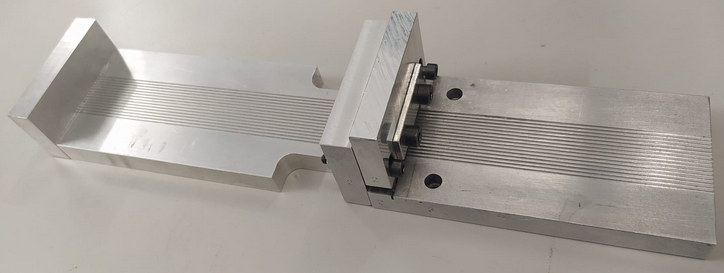
\includegraphics[width=\textwidth]{12Summary/4ResearchAndDevelopments/41Fibers/CuttingDeviceVS.png}  
    \caption{\label{subfig:MaquinaTallar}}
    \end{subfigure}
    \hfill
    \begin{subfigure}[b]{0.45\textwidth}
    \centering
    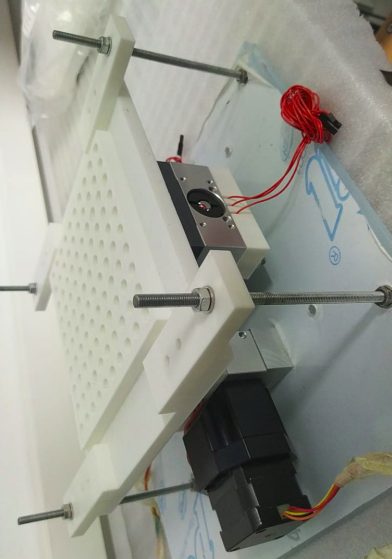
\includegraphics[angle=-90, width=\textwidth]{12Summary/4ResearchAndDevelopments/41Fibers/PolishingTable1.png}  
    \caption{\label{subfig:MaquinaPolir}}
    \end{subfigure}
 \caption{Màquines desenvolupades al projecte TRITIUM per a a) tallar fibres centellejadores i b) polir fibres centellejadores en massa. \label{fig:MaquinesTRITIUM}}
\end{figure}